%!TEX program = xelatex

% 制作请参考:https://github.com/tuna/THU-Beamer-Theme/blob/master/slide.tex
% 以及:https://www.zhihu.com/question/29676847

% ---------------------------------------------------------------------
% 基本设定
\documentclass[aspectratio=169]{beamer}
\usepackage{ctex}
\usepackage[T1]{fontenc}

% 说明:基于2019级大佬石寰宇的模板进行魔改,详见https://zhuanlan.zhihu.com/p/620722147;在此特别感谢大佬的工作!
% 魔改参考了:https://www.zhihu.com/question/29676847
% 说明:本设定用于Beamer制作。



% ---------------------------------------------------------------------
% 自定义颜色
% Firefly配色!!!
\usepackage{xcolor}
\definecolor{c1}{HTML}{3E324A} % #3e324a(紫黑)
\definecolor{c2}{HTML}{475D7B} % #475d7b(灰蓝)
\definecolor{c3}{HTML}{97C6C0} % #97c6c0(灰绿)
\definecolor{c4}{HTML}{E26E1B} % #e26e1b(深橘红)
\definecolor{c5}{HTML}{E6E4E0} % #e6e4e0(银白)
\definecolor{c6}{HTML}{4DF8E8} % #4df8e8(蓝绿)
\definecolor{c7}{HTML}{C2D5CD} % #c2d5cd(茉绿)


% ---------------------------------------------------------------------
% 设置主题颜色

% 方式1
% 用这一个:\documentclass{beamer}\usetheme{Madrid}
%\usecolortheme[named=c1]{structure}
%\setbeamercolor{frametitle}{fg=c2, bg=c6}
%\setbeamercolor{item}{fg=c3}
%\setbeamercolor{item projected}{fg=c1}
%\setbeamercolor{title}{fg=c2, bg=c6}


% 方式2
% 采用方式二就不要用主题;下面魔改了一个空白的主题
% 用这一个:\documentclass[aspectratio=169]{beamer}
% 加导航条
\useoutertheme[width=3\baselineskip,right]{sidebar}
%\useoutertheme[width=3\baselineskip,left]{sidebar}
\setbeamercolor{section in sidebar}{fg=c2, bg=c3}
%\setbeamercolor{section in sidebar}{fg=c2, bg=c6}
%\setbeamerfont{section in sidebar}{series=\bfseries}
% 目录标数字
\setbeamertemplate{section in toc}[sections numbered] 
%\setbeamertemplate{subsection in toc}[subsections numbered]
%\setbeamertemplate{subsubsection in toc}[subsubsections numbered]
% 无序列表用实心点
\setbeamertemplate{itemize item}{$\bullet$}
\setbeamertemplate{enumerate item}{\textbf{\insertenumlabel}.}
% 去掉下面没用的导航条
\setbeamertemplate{navigation symbols}{}
% 设置页脚格式
\makeatother
\setbeamertemplate{footline}
{
	\leavevmode%
	\hbox{%
		\begin{beamercolorbox}[wd=.4\paperwidth,ht=2.25ex,dp=1ex,center]{author in head/foot}%
			\usebeamerfont{author in head/foot}\insertauthor
		\end{beamercolorbox}
		
		\begin{beamercolorbox}[wd=.6\paperwidth,ht=2.25ex,dp=1ex,center]{title in head/foot}%
			\usebeamerfont{title in head/foot}\inserttitle\hspace*{13em}
			\insertframenumber{} / \inserttotalframenumber\hspace*{0ex}
	\end{beamercolorbox}}
	
	\vskip0pt%
}
\makeatletter
% 不同元素指定不同颜色,fg是本身颜色,bg是背景颜色,!num!改变数值提供渐变色
\setbeamercolor{title}{fg=c2, bg=c5}
\setbeamercolor{frametitle}{fg=c2, bg=c5}
% 设置页脚对应位置颜色
\setbeamercolor{author in head/foot}{fg=c5, bg=c1}
\setbeamercolor{title in head/foot}{fg=c5, bg=c1}
% 设置sidebar颜色
%\setbeamercolor{sidebar right}{bg=c7}
\setbeamercolor{sidebar right}{bg=c5}
%\setbeamercolor{sidebar left}{bg=c7}
\setbeamercolor{structure}{fg=c2, bg=c3} 
\setbeamercolor{item}{fg=c6}
% 左右页间距的排版
\def\swidth{2.3cm}
%\setbeamersize{sidebar width right=\swidth}
%\setbeamersize{sidebar width left=\swidth}
\setbeamersize{sidebar width right=1.8cm}
\setbeamersize{sidebar width left=1.8cm}
\setbeamerfont{title in sidebar}{size=\scriptsize}
\setbeamerfont{section in sidebar}{size=\tiny}


% ---------------------------------------------------------------------
% 引入必要的包
\usepackage{amsmath,enumerate,multirow,float}
\usepackage{tabularx}
\usepackage{tabu}
\usepackage{subfig}
\usepackage{fancyhdr}
\usepackage{graphicx}
\usepackage{wrapfig}  
\usepackage{physics}
\usepackage{appendix}
\usepackage{amsfonts}

\usepackage{mathrsfs} % 字体
\usepackage{calligra}
\usepackage{lipsum}
\usepackage{adjustbox}
\usepackage{tabularray} % 绘制表格时可以更加方便添加框线

% ---------------------------------------------------------------------
% 颜色盒子
\usepackage{tcolorbox}
\tcbuselibrary{skins,breakable}

\newtcolorbox[auto counter,number within=section]{myhighlight}[1][]{
  top=2pt,bottom=2pt,arc=1mm,
  boxrule=0.5pt,
%   frame hidden,
  breakable,
  enhanced, %跨页后不会显示下边框
  coltitle=c2!80!gray,
  colframe=c3,
  colback=c6,
  drop fuzzy shadow,
  title={Key Point~\thetcbcounter:\quad},
  fonttitle=\bfseries,
  attach title to upper,
  #1
}



% ---------------------------------------------------------------------
% 利用cleveref改变引用格式,\cref是引用命令
\usepackage{cleveref}
\crefformat{figure}{#2{\textcolor{c2}{\textbf{Figure #1}}}#3} % 图片的引用格式
\crefformat{equation}{#2{(\textcolor{c2}{#1})}#3} % 公式的引用格式
\crefformat{table}{#2{\textcolor{c2}{\textbf{Table #1}}}#3} % 表格的引用格式



% ---------------------------------------------------------------------
%	对目录、章节标题的设置
%\usepackage{hyperref} 
%\hypersetup{
%	colorlinks,
%	linktoc = section, % 超链接位置,选项有section, page, all
%	linkcolor = c2, % linkcolor 目录颜色
%	citecolor = c2  % citecolor 引用颜色
%}


% ---------------------------------------------------------------------
%   listing代码环境设置
\usepackage{listings}
\lstloadlanguages{python}
\lstdefinestyle{pythonstyle}{
backgroundcolor=\color{gray!5},
language=python,
frameround=tftt,
frame=shadowbox, 
keepspaces=true,
breaklines,
columns=spaceflexible,                   
basicstyle=\ttfamily\small, % 基本文本设置,字体为teletype,大小为scriptsize
keywordstyle=[1]\color{c1}\bfseries, 
keywordstyle=[2]\color{Red!70!black},   
stringstyle=\color{Purple},       
showstringspaces=false,
commentstyle=\ttfamily\scriptsize\color{green!40!black},%注释文本设置,字体为sf,大小为smaller
tabsize=2,
morekeywords={as},
morekeywords=[2]{np, plt, sp},
numbers=left, % 代码行数
numberstyle=\it\tiny\color{gray}, % 代码行数的数字字体设置
stepnumber=1,
rulesepcolor=\color{gray!30!white}
}



% ---------------------------------------------------------------------
%	其他设置
\def\degree{${}^{\circ}$} % 角度
\graphicspath{{./images/}} % 插入图片的相对路径
\allowdisplaybreaks[4]  %允许公式跨页

\captionsetup[figure]{name=Figure} % 图片形式
\captionsetup[table]{name=Table} % 表格形式 

% Define a counter
\newcounter{currentenumi}

%---------------------------------------------------------------------
%	正文
%---------------------------------------------------------------------



\begin{document}
%---------------------------------------------------------------------
%---------------------------------------------------------------------
%---------------------------------------------------------------------		
	
	
	% 个人信息
	\author[]{戴鹏辉 \& 杨舒云}
	\title[]{基于热电效应的热机设计与热力学第二定律验证实验}
	\subtitle{设计性实验“热力学第二定律”开题报告}
	\date{May 16, 2024}
	%---
	
	
	% 封面
	\frame[plain]{\titlepage}
	% ---
	
	
	% 总目录
	\begin{frame}
		\frametitle{Outline}
		\tableofcontents
	\end{frame}
	% ---
	
	
	% 第一章
	\section{回顾实验要求}
	
	% 章目录
	\frame{\frametitle{Outline}\tableofcontents[currentsection]}
	
	% 内容
	\begin{frame}
		\frametitle{回顾实验要求I}
		
		\begin{block}{目的}
			设计并实现输出功率在1瓦以上的“热机”,以探究和验证热力学第二定律。
		\end{block}
		
	\end{frame}	
	
	\begin{frame}
		\frametitle{回顾实验要II}
		
		\begin{block}{要求}
			\begin{enumerate}
				\item \textbf{学习和理解热电效应}:
				\begin{itemize}
					\scriptsize \item 包括Seebeck效应、Peltier效应和Thomson效应。
					\item \scriptsize 设计实验方案,包含原理和物理模型。
				\end{itemize}
				
				\item \textbf{制作热机}:
				\begin{itemize}
					\scriptsize \item \scriptsize 展示热力学第二定律的“热机”。
					\item \scriptsize 电或机械输出功率不低于1瓦。
				\end{itemize}
				
				\item \textbf{测量与分析}:
				\begin{itemize}
					\scriptsize \item \scriptsize 测量装置的最大输出功率和输出效率。
					\item \scriptsize 讨论实际结果与Carnot循环的差异。
					\item \scriptsize 探讨进一步提高效率的方法。
					\item \scriptsize 分析测量精度和不确定度。
				\end{itemize}
				
				\item \textbf{确保安全性}:
				\begin{itemize}
					\scriptsize \item \scriptsize 确保装置表面(可触摸到的部分)温度不高于50\degree C。
				\end{itemize}
			\end{enumerate}
		\end{block}
	\end{frame}
	
	\begin{frame}
		\frametitle{回顾实验要求III}
		
		\begin{block}{熟悉基本实验装置,搭建与操作}
			\begin{itemize}
				\item \textbf{开路输出电压与温差的关系}:
				\begin{itemize}
					\item Seebeck效应,器件的等效热电系数 $\alpha$ 和等效热导 $\lambda$(热阻 $\rho$)。
				\end{itemize}
				
				\item \textbf{特定负载下输出功率与温差的关系}:
				\begin{itemize}
					\item 验证热力学第二定律。
				\end{itemize}
				
				\item \textbf{热源功率和单片热电堆输出效率的优化}:
				\begin{itemize}
					\item 在给定热源功率下,优化室温条件下单片热电堆的输出效率。
				\end{itemize}
				
				\item \textbf{固定冷、热源温度下的测量}:
				\begin{itemize}
					\item 测量在不同负载下的热电机输出功率与输出效率的关系。
					\item 分析器件内阻 $r$。
				\end{itemize}
			\end{itemize}
		\end{block}
	\end{frame}
	
	% ---
	
	
	% 第二章
	\section{实验原理概述}
	
	% 章目录
	\frame{\frametitle{Outline}\tableofcontents[currentsection]}
	
	% 内容
	\begin{frame}
		\frametitle{实验原理概述:三种热电效应I}
		
		\begin{block}{Seebeck效应}
			\small 当两种不同的导体或半导体连接成回路,并且两个接头的温度不同,就会在回路中产生\textcolor{c4}{电动势}。
			
			\begin{figure}[htbp]
				\centering
				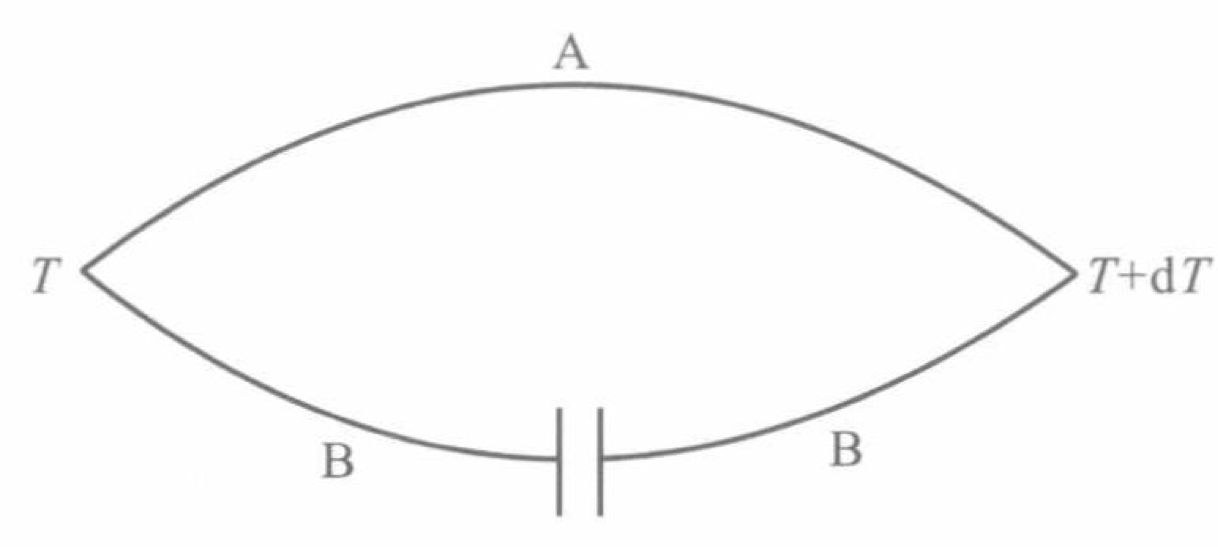
\includegraphics[width=0.45\textwidth]{SamPre_1_Gra1.jpg}
			\end{figure}
			
			\begin{myhighlight}
				$$\mathrm{d}V=\epsilon_{AB}\mathrm{d}T$$
			\end{myhighlight}
			\footnotesize 其中,$\epsilon_{AB}$是温差电动势系数(又称\textcolor{c4}{Seebeck系数},记为$\alpha$)。符号约定为如果在高温段电动势驱使电流由金属A流向金属B为正。			
		\end{block}
		
	\end{frame}
	
	\begin{frame}
		\frametitle{实验原理概述:三种热电效应II}
		
		\begin{block}{Peltier效应}
			\small 当电流通过两种不同材料组成的电路时,一个接头会吸热,另一个接头会放热。这个效应对于\textcolor{c4}{调控热机的温度}非常重要,尤其是在确保装置表面温度不超过50\degree C的安全要求下。
			
			\begin{figure}[htbp]
				\centering
				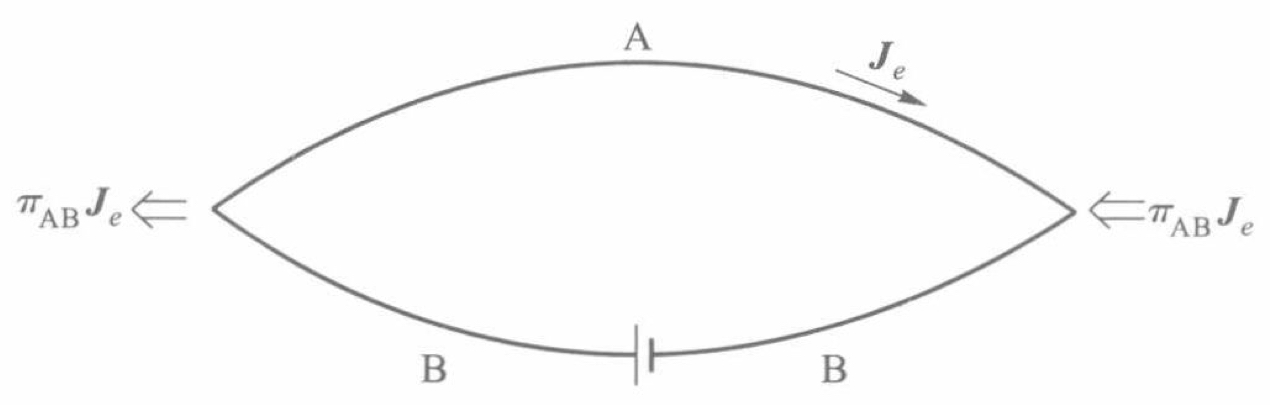
\includegraphics[width=0.5\textwidth]{SamPre_1_Gra2.jpg}
			\end{figure}
			
			\begin{myhighlight}
				$$\textbf{J}_{q\pi}=\pi_{AB}\textbf{J}_{e}$$
			\end{myhighlight}
			\footnotesize 其中,$\textbf{J}_{q\pi}$是Peltier热流密度,$\textbf{J}_{e}$是从A到B的电流密度,$\pi_{AB}$是两种金属的Peltier系数(与温度有关)。
		\end{block}
		
	\end{frame}
	
	\begin{frame}
		\frametitle{实验原理概述:三种热电效应III}
		
		\begin{block}{Thomson效应}
			\scriptsize 在均质导体中,如果存在温度梯度,当电流通过时,会伴随着吸热或放热的现象。这对于完整的热电模型和效率分析很关键。$\dot{Q}=\mu I\cdot \nabla T$,$\mu$为Thomson系数。
		\end{block}
		
		\begin{block}{热电模型参数}
			\begin{itemize}
				\scriptsize \item \scriptsize 等效热导表示材料传导热量的能力,单位通常为瓦每米每开尔文(W/m·K)。等效热导越大,材料的热传导能力越强。
				$
				\lambda = \frac{Q}{A \cdot \Delta T \cdot t}
				$。
				\scriptsize 其中,$\lambda$ 是等效热导(W/m·K),$Q$ 是通过材料的热量(J),$A$ 是材料的横截面积($m^2$),$\Delta T$ 是材料两端的温差(K),$t$ 是热量传导所需的时间(s)。
				\scriptsize 通过Fourier热传导定律,也可以表示为(其中 $L$ 是材料的长度(m)):
				$
				Q = \lambda \cdot A \cdot \frac{\Delta T}{L} \cdot t
				$。
				
				\item \scriptsize 热阻表示材料对热流阻碍的能力,单位通常为开尔文每瓦(K/W)。热阻越大,材料的热流阻碍能力越强。
				$
				R_{\text{th}} = \frac{\Delta T}{Q}
				$。
				\scriptsize 其中,$R_{\text{th}}$ 是热阻(K/W),$\Delta T$ 是材料两端的温差(K),$Q$ 是通过材料的热量(W)。
				
				\item \scriptsize 等效热导和热阻是互为倒数的关系:
				$
				R_{\text{th}} = \frac{L}{\lambda \cdot A}
				$,
				$
				\lambda = \frac{L}{R_{\text{th}} \cdot A}
				$。
			\end{itemize}
		\end{block}
		
	\end{frame}
	
	\begin{frame}
		\frametitle{实验原理概述:输出电路部分}
		
		\begin{block}{Seebeck效应电源的外输出特性}
			\begin{itemize}
				\item 开路电压是指没有外部负载连接时,热电发电装置两端的电压。根据Seebeck效应,开路电压与温差成正比,$V_{\text{oc}} = \alpha \Delta T$。
				
				\item 当热电发电装置连接到负载时,输出电压会由于内阻的存在而下降。负载电压$V_{\text{L}} = \frac{\alpha \Delta T \cdot R_{\text{L}}}{R_{\text{L}} + R_{\text{in}}}$,而输出功率是负载上消耗的功率$P_{\text{out}} = \frac{(\alpha \Delta T)^2 \cdot R_{\text{L}}}{(R_{\text{L}} + R_{\text{in}})^2}$。
				
				\item \textcolor{c4}{当负载电阻等于内阻时},热电发电装置输出的功率达到最大$P_{\text{max}} = \frac{(\alpha \Delta T)^2}{4 R_{\text{in}}}$。				
			\end{itemize}						
		\end{block}
		
	\end{frame}
	
	\begin{frame}
		\frametitle{实验原理概述:电加热器}
		
		\begin{block}{电加热器的工作原理}
			电加热器(电热贴)通过电能转化为热能来实现加热,其工作原理基于焦耳定律$Q = I^2 R t$。
		\end{block}
		
		\begin{block}{加热功率的测量}
			使用电压表并联连接在电加热器两端,读取电压值;使用电流表串联连接在电路中,读取电流值;根据测得的电压和电流,使用公式$P = VI$计算加热功率。
			
			或者采用使用欧姆表测量电加热器的电阻,使用测得的电阻和电流计算$P = I^2 R$。
			
			对于电流电压随时间变化的情况,计算一段时间的总热功可以利用\textcolor{c4}{积分}来实现。
		\end{block}
		
	\end{frame}
	
	\begin{frame}
		\frametitle{实验原理概述:PID控温I}
		\begin{block}{控温算法}
			
			\begin{table}[h]
				\centering
				%\label{tab:tab1}
				%\caption{高级控温算法的比较}
				\resizebox{\textwidth}{!}{%
				\begin{tabular}{|c|c|c|}
					\hline
					控温算法 & 优点 & 缺点 \\
					\hline
					\textcolor{c4}{PID 控制} & 简单、易实现 & 性能有限,难以处理复杂系统 \\
					\hline
					模糊控制 & 不需要精确模型,适应性强 & 规则设计复杂,性能依赖于规则质量 \\
					\hline
					模型预测控制 & 最优性能,多变量处理 & 计算量大,依赖系统模型 \\
					\hline
					自适应控制 & 参数自调整,适应性强 & 实现复杂,收敛性问题 \\
					\hline
					神经网络控制 & 非线性处理能力强 & 训练复杂,数据需求大 \\
					\hline
					最优控制 & 理论性能优 & 实现复杂,计算量大 \\
					\hline
				\end{tabular}
			}				
			\end{table}
			
		\end{block}
	\end{frame}
	
	\begin{frame}
		\frametitle{实验原理概述:PID控温II}
		
		\begin{block}{先考虑采用最经典的PID控温}
			\begin{itemize}
				\small\item PID(Proportional-Integral-Derivative)控制是一种用于温度控制的经典算法,通过对误差的比例、积分和微分进行计算和调整,精确控制加热器的输出,从而实现温度的稳定控制。PID 控制器通常由三个部分组成:比例(P),积分(I),和微分(D)。
				
				\small\item PID 控温的控制量 $u(t)$ 可以表示为:$$u(t) = K_p e(t) + K_i \int_0^t e(\tau) d\tau + K_d \frac{d e(t)}{dt}$$
				
				\item \small 比例控制$P_{\text{out}} = K_p e(t)$直接与当前误差成比例,调整系统响应速度;积分控制$I_{\text{out}} = K_i \int_0^t e(\tau) d\tau$对误差进行积分,消除稳态误差,增强系统的长期精度;微分控制$D_{\text{out}} = K_d \frac{d e(t)}{dt}$对误差进行微分,预测误差变化趋势,减小超调和振荡。
			\end{itemize}			
		\end{block}
		
	\end{frame}
	
	\begin{frame}
		\frametitle{实验原理概述:PID控温III}
		
		\begin{block}{离散形式的 PID 控制算法}
			在实际应用中,PID 控制通常以\textcolor{c4}{离散形式}实现。离散 PID 控制算法如下:			
			\begin{myhighlight}
				\small\[
				u[k] = u[k-1] + K_p (e[k] - e[k-1]) + K_i e[k] + K_d \left( \frac{e[k] - e[k-1]}{T} \right)
				\]
			\end{myhighlight}
			其中:
			\begin{itemize}
				\item $u[k]$ 是第 $k$ 次采样时的控制输出;
				\item $e[k]$ 是第 $k$ 次采样时的误差;
				\item $T$ 是采样周期。
			\end{itemize}
		\end{block}
		
	\end{frame}
	
	% ---
	
	
	% 第二章
	\section{实验方案}
	
	% 章目录
	\frame{\frametitle{Outline}\tableofcontents[currentsection]}
	
	% 内容
	\begin{frame}[allowframebreaks]
		\frametitle{实验方案:总体规划}
		
		\begin{enumerate}
			\item 各元件性能测量
			\begin{itemize}
				\item \textcolor{c4}{Seebeck效应测量}:通过改变温差并测量开路电压来研究Seebeck效应,从而确定$\alpha$;
				\item 器件内阻的测量与影响:内阻对热电转换效率有重要影响,了解并优化内阻对提高热机性能是必要的;
				\item 考虑测量电加热器的加热功率(以及其它元件性能,如Peltier效应)。
			\end{itemize}
			
			\item \textcolor{c4}{搭建热机}
				\begin{itemize}
					\item \textcolor{c4}{热电堆集成——电加热器与Seebeck元件,测控部分——PID控温(热端、冷端),输出电路部分(输出功率测量)。}
				\end{itemize}
			
			\item 负载与效率测量
			\begin{itemize}
				\item \textcolor{c4}{加热功率测控}——电流表电压表实时测控(含于PID系统中,编写相关程序);
				\item \textcolor{c4}{输出功率测控}——电流表电压表实时测控(考虑是否编程);
				\item 测量最大输出功率——改变输出电路的负载;
				\item 测量最大输出效率——改变温差与负载,优化其它部分;
				\item 探究如何测量热端的损失。
			\end{itemize}
			
			\item 热力学第二定律的展示
			\begin{itemize}
				\item \textcolor{c4}{通过实验测量,展示即使是优化过的热电装置,其效率也受到卡诺效率的限制,这直接体现了热力学第二定律。}
				\item 讨论如何通过实验设计来逼近卡诺效率,包括使用最佳材料、最佳温差和最佳负载条件。
			\end{itemize}			
			
			\item 结论与进一步的探索
			\begin{itemize}
				\item 比较热机效率与理论卡诺效率的差异,讨论可能的优化途径和技术挑战;
				\item 探究各部分如何\textcolor{c4}{优化}(热电堆——减小散热,增大温差,冷热端优化;测控——优化控温算法,改进实时测量程序;输出电路部分——减小散热,考虑Thomson效应的影响;理论建模——估算散热进一步修正)。
			\end{itemize}
		\end{enumerate}
		
		\begin{figure}[htbp]
			\centering
			\subfloat[]{
				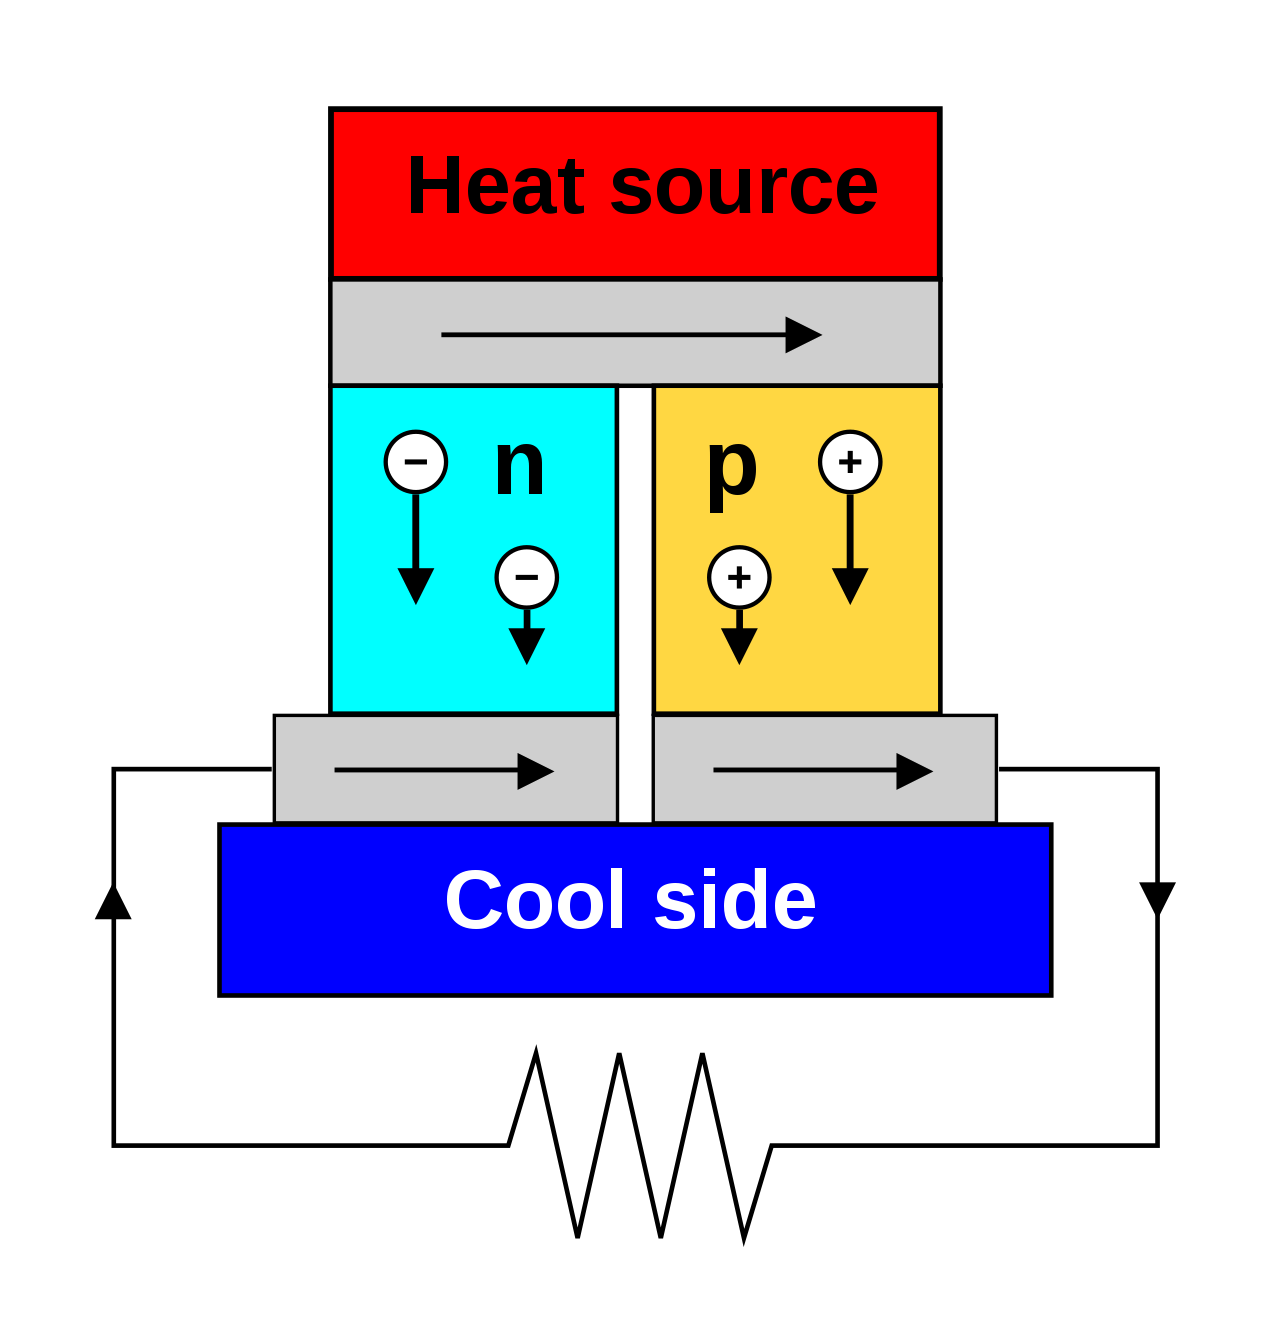
\includegraphics[width=0.33\textwidth]{SamPre_1_Gra3.png}
			}
			\subfloat[]{
				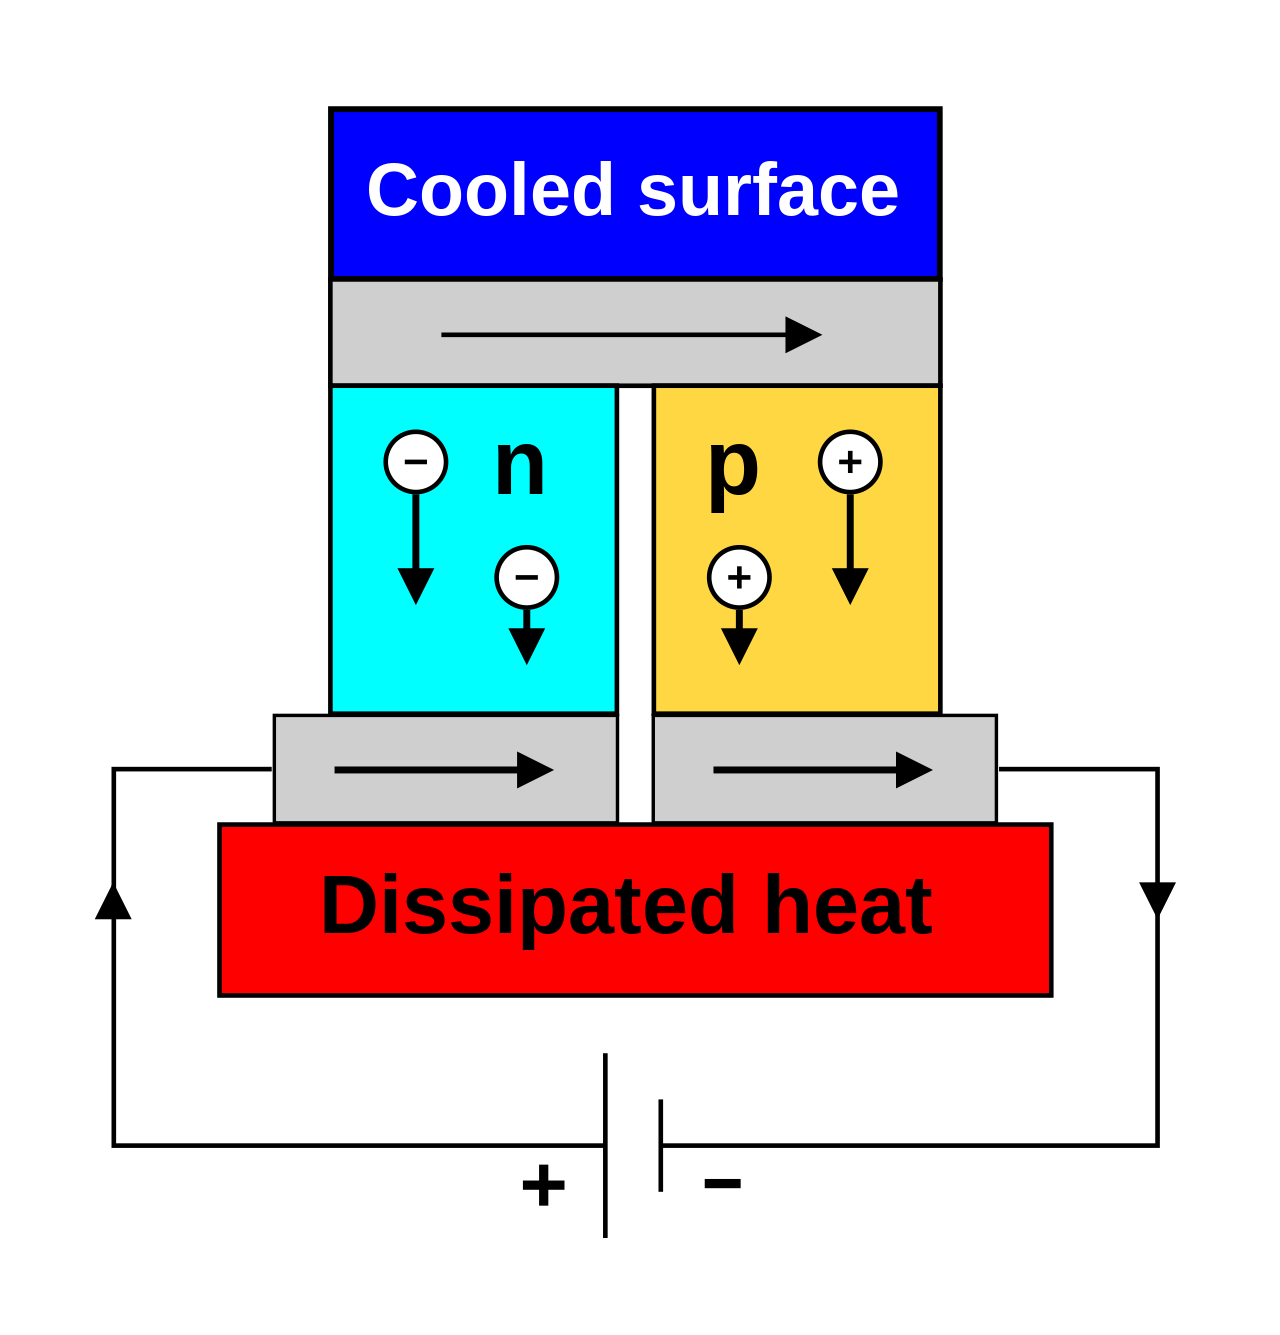
\includegraphics[width=0.33\textwidth]{SamPre_1_Gra4.png}
			}	
		\end{figure}
		
	\end{frame}
		
	\begin{frame}	
		\frametitle{实验方案:搭建热机I}
		
		\begin{block}{材料与组件}
			\begin{itemize}
				\small\item \textcolor{c4}{热电模块}:选择具有高Seebeck系数、低热导率的热电模块,比如基于铋锑合金(Bi2Te3)的商用模块。
				\item 热源:电加热器,可以提供稳定和可调的热量。
				\item \textcolor{c4}{冷却系统}:水冷散热器或大功率风扇(或者Peltier元件),用于冷却热电模块的冷端。
				\item 测量设备:电流表、电压表、功率计,用于测量输出电流、电压和功率。
				\item 温度传感器:用于监控热端和冷端的温度。
				\item 绝缘材料:用于隔热,确保热量集中传递给热电模块的热端。
				\item 负载:电阻或电阻箱,用作热机输出的负载,以测量其输出功率。
			\end{itemize}
		\end{block}
		
	\end{frame}
		
	\begin{frame}	
		\frametitle{实验方案:搭建热机II}	
		
		\begin{block}{搭建方案}
			\begin{enumerate}
				\item 热电模块配置:将若干热电模块串联,以增加输出电压。根据需要的输出功率和单个热电模块的性能,计算所需模块的数量。并联可以增加输出电流。
				
				\item 热源与冷却系统安装:
				\begin{itemize}
					\item \textcolor{c4}{将电加热器固定在热电模块的一侧作为热源,保证热端能够获得足够高的温度。}
					\item \textcolor{c4}{在热电模块的另一侧安装冷却系统,保持冷端的温度尽可能低。}
				\end{itemize}				
				
				\item 电气连接与测量:
				\begin{itemize}
					\item 将电压表和电流表并联/串联到热电模块或模块组合的输出端,以便测量输出电压和电流。
					\item 将负载连接到热电模块的输出端,开始时可以使用一个较高的电阻值作为基准。
				\end{itemize}
				
				% Store the actual item number
				\setcounter{currentenumi}{\theenumi}			
				
			\end{enumerate}
		\end{block}
		
	\end{frame}
	
	\begin{frame}	
		\frametitle{实验方案:搭建热机III}	
		
		\begin{block}{搭建方案}
			\begin{enumerate}
				
				% Use the previous stored item number
				\setcounter{enumi}{\thecurrentenumi}			
				
				\item 温度监控与安全保障:
				\begin{itemize}
					\item 在热端和冷端分别安装温度传感器,实时监控温度,确保热端温度在安全范围内,且冷端不会过热。
					\item 使用绝缘材料和防护措施确保操作者不会直接接触到高温部分。
				\end{itemize}
				
				\item 输出功率的测量与优化:
				\begin{itemize}
					\item 逐步调整负载电阻,测量不同负载条件下的输出功率,找到输出功率最大时的负载电阻值。
					\item 记录最优负载条件下的输出电压、电流和功率,验证是否达到或超过1W的输出。
				\end{itemize}
			\end{enumerate}
		\end{block}
		
	\end{frame}
	
	\begin{frame}
		\frametitle{实验方案:温度控制I}
		
		\begin{block}{思路}
			\begin{myhighlight}
				控制冷端与热端温度恒定 ,一方面可用于计算卡诺机效率,另一方面便于计算吸收热量。
			\end{myhighlight}
		\end{block}
		
		\begin{block}{整体方案}
			\begin{enumerate}
				\item 温度监测
				\begin{itemize}
					\item 在热端和冷端分别安装高精度的温度传感器,如热电偶或PT100传感器,以实时监测温度。
				\end{itemize}
				
				% Store the actual item number
				\setcounter{currentenumi}{\theenumi}
				
			\end{enumerate}
		\end{block}
	\end{frame}
	
	\begin{frame}
		\frametitle{实验方案:温度控制II}
		
		\begin{block}{整体方案}
			\begin{enumerate}
				
				% Use the previous stored item number
				\setcounter{enumi}{\thecurrentenumi}
				
				\footnotesize\item 热端温度控制
				\begin{itemize}
					\footnotesize\item 可控加热源:使用可调节的加热设备(如电加热器)来精确控制热端温度。结合\textcolor{c4}{PID控制器}可以根据温度传感器的反馈自动调整加热功率,以保持目标温度。
					\footnotesize\item \textcolor{c4}{隔热材料}:在热端周围使用高效的隔热材料减少热损失,有助于维持稳定的温度。
				\end{itemize}
				
				\footnotesize\item 冷端温度控制
				\begin{itemize}
					\footnotesize\item 主动冷却系统:将另一个温度传感器安装在冷端,将其输出连接到控制冷端温度的\textcolor{c4}{PID控制器}。对于Peltier制冷方案,PID控制器的输出控制Peltier元件的工作电流。对于水冷方案,PID控制器调节水泵的流速或风扇的转速,根据冷端温度与目标温度的偏差来调整冷却强度,维持冷端温度。
					
					\footnotesize\item 热管理策略:优化散热器的设计(如增加散热片、使用热管技术),以提高冷端的散热效率。
				\end{itemize}
	
			\end{enumerate}
		\end{block}
	\end{frame}
	
	\begin{frame}
		\frametitle{实验方案:测量热机效率}
		
		\begin{enumerate}
			\item 测量输出电功率
			\begin{itemize}
				\item 使用电流表和电压表测量热电模块(和电加热器)的输出电流(I)和电压(V)。 
			\end{itemize}
			
			\item 测量输入热功率
			\begin{itemize}
				\item 直接法:如果使用热流计,直接测量输入到热机的热流量(Q)。然后,根据加热源工作的时间(t),计算输入的热功率。
				\item 间接法:如果没有热流计,\textcolor{c4}{可以通过测量加热源的电功率和效率来估算输入的热功率}。
			\end{itemize}
			
			\item \textcolor{c4}{测量温度差}
			\begin{itemize}
				\item 使用温度传感器测量热端和冷端的温度,以评估热机工作的温度差。
			\end{itemize}
			
			\item 计算效率
			\begin{itemize}
				\item 使用测得的电功率和热功率计算热机的效率。
			\end{itemize}
		\end{enumerate}
	\end{frame}
	
	\begin{frame}
		\frametitle{实验方案:优化}
		
		\begin{itemize}
			\item 热电耦合:通过改进热电模块两端的热交换设计,如使用高效热交换材料和技术(如\textcolor{c4}{微通道冷却}),可以提高热端和冷端的温度梯度,进一步提升效率。
			
			\item \textcolor{c4}{多级热电堆}设计:通过串联多个热电模块,形成多级热电堆,可以在更大的温差下工作,提高整体转换效率。但这需要精密的温度和电流管理。
			
			\item 散热系统优化:\textcolor{c4}{优化冷端的散热设计},可以是通过增加散热片面积、改进风扇布局或采用液冷系统,以提高热电堆的冷却效率。
			
			\item 整体系统设计:\textcolor{c4}{在系统级别上考虑热电堆的集成},包括电源管理、热管理和控制策略的优化,可以进一步提升效率。
		\end{itemize}
		
	\end{frame}
	
	% ---
	
	
	% 致谢
	\begin{frame}[plain]
		
		\begin{center}
			{\Huge\calligra Thanks for listening!}
		\end{center}
		
	\end{frame}
	
	
	
	
	
	
	
%---------------------------------------------------------------------	
%---------------------------------------------------------------------
%---------------------------------------------------------------------
\end{document}